\documentclass[12pt]{kiarticle} % You can learn about my document class "kiarticle" and install it to your device by following the link: https://github.com/Kiarendil/toolkitex
\graphicspath{{pictures/}}
\DeclareGraphicsExtensions{.pdf,.png,.jpg,.eps}
%%%
\pagestyle{fancy}
\fancyhf{}
%\renewcommand{\headrulewidth}{ 0.1mm }
\renewcommand{\footrulewidth}{ .0em }
\fancyfoot[C]{\texttt{\textemdash~\thepage~\textemdash}}
\fancyhead[L]{Лабораторная работа № 6.1 \hfil}
\fancyhead[R]{\hfil Иванов Кирилл, 625 группа }
\usepackage{multirow} % Слияние строк в таблице
\newcommand
{\un}[1]
{\ensuremath{\text{#1}}}
\newcommand{\eds}{\ensuremath{ \mathscr{E}}}
\usepackage{tikz}
%%% Работа с таблицами
\usepackage{array,tabularx,tabulary,booktabs} % Дополнительная работа с таблицами
\usepackage{longtable}  % Длинные таблицы
\usepackage{multirow} % Слияние строк в таблице

\begin{document}
	
	\begin{titlepage}
	\begin{center}
		\large 	Московский физико-технический институт \\
		(государственный университет) \\
		Факультет общей и прикладной физики \\
		\vspace{0.2cm}
		
		\vspace{4.5cm}
		Лабораторная работа № 6.1 \\ \vspace{0.2cm}
		\large (Общая физика: квантовая физика) \\ \vspace{0.2cm}
		\LARGE \textbf{Эффект Мессбауэра}
	\end{center}
	\vspace{2.3cm} \large
	
	\begin{center}
		Работу выполнил: \\
		Иванов Кирилл,
		625 группа
		\vspace{10mm}		
		
	\end{center}
	
	\begin{center} \vspace{60mm}
		г. Долгопрудный \\
		2018 год
	\end{center}
\end{titlepage}
	
	\paragraph*{Цель работы:} С помощью метода доплеровского сдвига мессбауэровской линии поглощения исследовать резонансное поглощение $ \gamma $-лучей, испускаемых
	ядрами олова $ ^{119} $ Sn в соединении BaSnO$_3$ при комнатной температуре.
	Определить положение максимума резонансного поглощения, его величина, а также экспериментальная ширина линии $ \Gamma_{экс}$. Оценить время жизни возбуждённого состояния ядра  $^{119}$Sn .
	
	\paragraph*{Оборудование:} 
	
	\section{Теоретическое введение} 
	
	\subsection{Испускание и поглощение в свободных атомах}
	
	\begin{wrapfigure}[20]{l}{0.35\linewidth}
		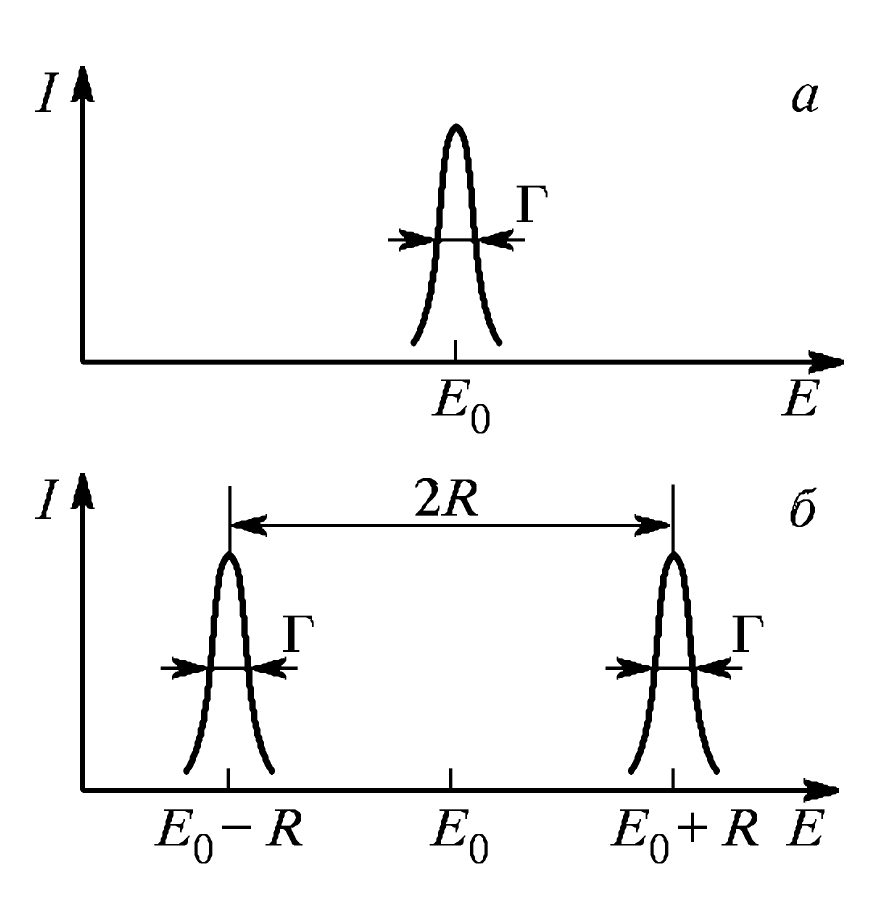
\includegraphics[width=\linewidth]{G}
		\caption{Энергетическое распределение, характеризующее возбужденное состояние ядра (а),
			и сдвиг линий испускания и поглощения из-за отдачи при свободных ядрах (б)}
		\label{ris 1}
	\end{wrapfigure}
	
	Нуклоны (нейтроны и протоны) в атомном ядре, как и электроны
	в атоме, могут находиться в различных дискретных энергетических
	состояниях, или, как говорят, на различных энергетических уровнях.
	Самый низкий из уровней называется основным, остальные носят название возбужденных. Ядра, находящиеся в возбужденных состояниях, могут переходить на более низкие энергетические уровни, в том
	числе и на основной уровень. Такие переходы происходят самопроизвольно (спонтанно). Освобождающаяся энергия уносится фотоном.
	Так возникает $ \gamma $-излучение.
	
	Ядра атомов могут не только испускать, но и поглощать фотоны. Если попадающий в атомное ядро фотон имеет
	энергию, равную разности энергий между основным и каким-либо возбужденным состояниями, то ядро может поглотить фотон и перейти в соответствующее возбужденное состояние. Этот процесс возможен лишь для $ \gamma $-лучей определенных энергий и носит, таким образом, резонансный характер.
	
	На первый взгляд резонансное поглощение  $ \gamma $-лучей должно представлять собой распространенное и легко наблюдаемое явление. Казалось бы, для его обнаружения достаточно пропустить поток $ \gamma $-лучей,
	испущенных радиоактивным источником, через поглотитель, содержащий те же ядра в невозбужденном состоянии. На самом деле это не так. Дело в том, что энергия $E_\gamma $, уносимая $ \gamma $-квантом, оказывается
	меньше энергии $ E_0 $ перехода между уровнями. Небольшая, но вполне
	заметная доля энергии уносится ядром, которое вследствие отдачи начинает двигаться в сторону, противоположную направлению вылета
	$ \gamma $-кванта.
	
	При испускании фотона ядро приобретает энергию отдачи
	
	\begin{equation}\label{R}
	R = \dfrac{p^2}{2M} = \dfrac{E_\gamma^2}{2Mc^2}
	\end{equation}
	
	Для ядра $ ^{119} $Sn, который используется в работе, $E_0 \backsimeq E_\gamma = 23,8 \; кэВ, \; R \backsimeq 2,5 \x 10^{-3} \; эВ \gg \Gamma/2 \backsimeq 3 \x 10^{-8} \; эВ $, где $ \Gamma $ --- естественная ширина линии. Из-за такой разницы в порядках величин получается, что при смещении на величину $ \pm R $ не перекрываются. Однако, это можно компенсировать эффектом Доплера, который возникает из-за теплового движения ядер. Для этого ядра должны двигаться относительно друг друга со скоростью
	
	\begin{equation}\label{V}
	V = c \dfrac{2R}{E_\gamma}
	\end{equation}
	 Это примерно 60 м/с для $ ^{119} $Sn. Из термодинамических соображений оценим скорость движения ядра $ v $:
	
	\begin{equation}\label{}
	\dfrac{Mv^2}{2} = \dfrac{kT}{2} \te v = \sqrt{\dfrac{kT}{M}}
	\end{equation}
	
	Тогда величину $ D $ доплеровского "<уширения"> линии с учетом \eqref{R} можно оценить как
	
	\begin{equation}\label{D}
	D = \dfrac{v}{c} E_\gamma = \sqrt{2RkT}
	\end{equation}
	
	При комнатной температуре для $ ^{119} $Sn эта величина будет примерно равна $ 1,5 \x 10^{-2} $ эВ, что на порядок больше $ R $. Происходит перекрытие линий испускания и поглощения вследствие доплеровского уширения. Это обеспечивает возможность резонансного поглощения гамма-лучей.
	
	\subsection{Испускание и поглощение в твердых телах}
	
	Совсем иначе обстоит дело в твердых телах --- в тех веществах с кристаллической решеткой, у которых энергия связи .между атомами в решетке больше энергии отдачи. В таком случае при испускании/поглощении импульс  в том или ином виде передается всем атомам в решетке, что часто вызвает ее колебания. Можно также сказать, что создаются кванты звуковых колебаний --- фононы. 
	
	В данной работе изучается \textbf{эффект Мессбауэра --- испускание и поглощение $ \gamma $-квантов без создания фононов (звуковых колебаний).} Его вероятность выражается формулой 
	
	\begin{equation}\label{}
	f = \exp{-\dfrac{4\pi \langle u^2 \rangle}{\lambda^2}}
	\end{equation}
	
	где $ \langle u^2 \rangle $ --- среднеквадратичное смещение ядер в процессе тепловых колебаний решетки (в направлении вылета $ \gamma $-кванта), $ \lambda $ --- длина волны $ \gamma $-излучения. Таким образом, вероятность упругого испускания (и поглощения) $ \gamma $-квантов уменьшается с температурой (с ростом $  \langle u^2 \rangle $) и с ростом энергии перехода (с уменьшением длины волны $ \lambda $).
	
	Расчеты показывают, что для наблюдения эффекта энергия фотонов должна быть порядка 200 кэВ. Температурный порог может быть разным; в изучаемых нами ядрах олова $ ^{119} $ Sn в соединении BaSnO$_3$ это возможно и при комнатной температуре. Для наблюдения эффекта гамма-излучение сначала пропускается через резонансный поглотитель со стабильными ядрами $ ^{119} $ Sn. Пройдя через него, излучение регистрируется сцинтилляционным спектрометром.  
	
	Наблюдение резонансного поглощения основано на методе доплеровского сдвига линий испускания и поглощения. Для этого поглотителю придается небольшая скорость, рассчитанная по формуле \eqref{V}, где вместо $ R $ подставлена $ \Gamma $. Мессбауэровская линия очень узка, и для наблюдения резонанса хватает скорости порядка миллиметра в секунду. 
	
		\begin{figure}[h!]
		\centering
			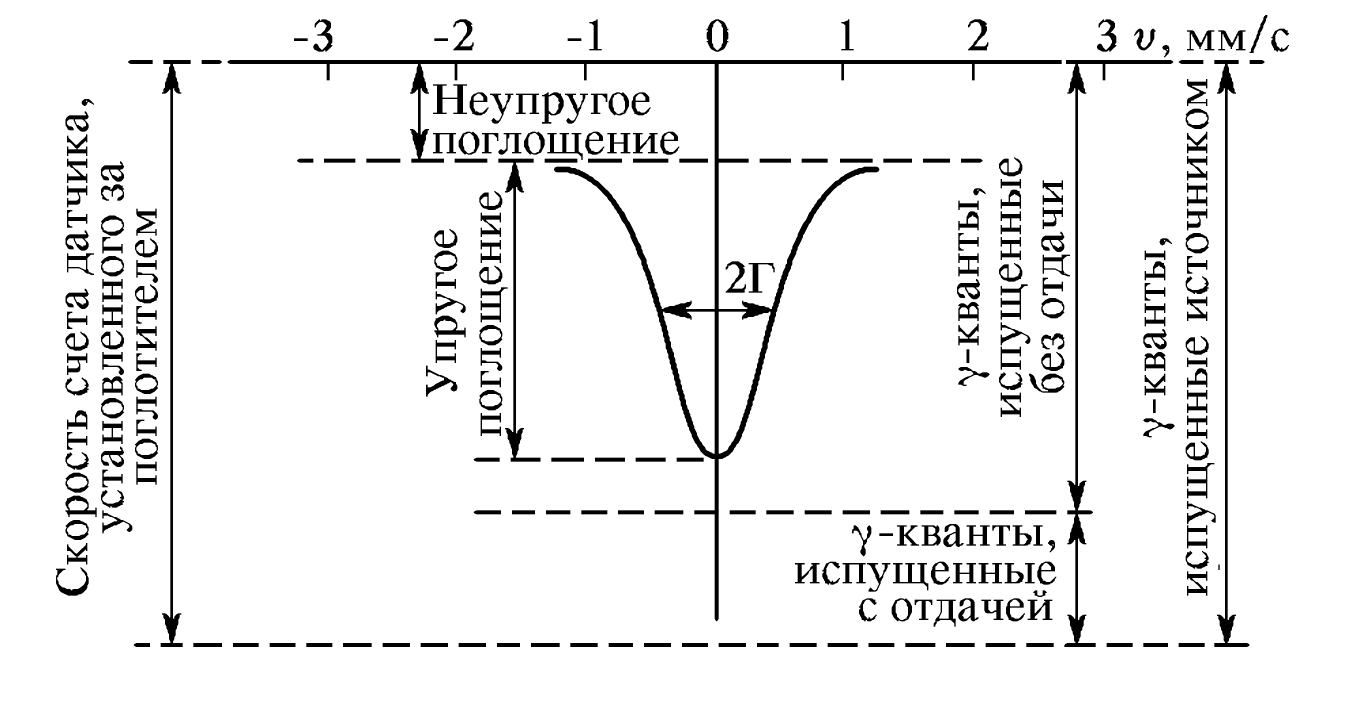
\includegraphics[width=0.7\linewidth]{spektr}
		\caption{Спектр упругого резонансного поглощения $ \gamma $-квантов. Источник и поглотитель находятся в идентичных кристаллических решетках. Неупругое поглощение
			обусловлено главным образом взаимодействием $ \gamma $-лучей с атомными электронами}
		\label{ris 2}
	\end{figure}
	
	Вообще говоря, при идентичных кристаллических решетках, линия испускания полностью перекрывается с линией поглощения, и максимальное поглощение
	наблюдается при нулевой скорости (рис. \ref{ris 2}). Однако в химических сплавах (как наш BaSnO$_3$) из-за влияния электростатических сил происходит смещение максимума поглощения, и его можно "<поймать"> при отличной от нуля скорости. Такое смещение называется \textbf{химическим сдвигом}. Его можно рассчитать по формуле 
	
	\begin{equation}\label{vr}
	v_p = \dfrac{\Delta E}{E_0}c
	\end{equation}
	
	Для подсчета "<амплитуды"> эффекта Мессбауэра обычно определяется безразмерная величина
	
	\begin{equation}\label{epsi;on}
	\epsilon(v) = \dfrac{N (\infty) - N(v)}{N (\infty) - N_ф}
	\end{equation}
	
	где $ N(v) $ --- скорость счета квантов, прошедших через поглотитель при
	некоторой скорости $ v $, $ N (\infty) $ --- скорость счета квантов при достаточно
	большой скорости, когда резонансное поглощение отсутствует, $ N_ф  $ --- скорость счета радиоактивного фона.
	
	Измеряемая на опыте ширина резонансной линии $  \Gamma_{экс} $ --- результат наложения линий источника и поглотителя. При тонких поглотителях и источниках и при отсутствии вибраций ширина линии равна удвоенной естественной ширине $ 2\Gamma $ (см. рис. \ref{ris 2}).
	
	На рис. \ref{ris 2} кривая задается формулой Брейта-Вигнера (лоренцева кривая):
	
	\begin{equation}\label{B-V}
	\sigma(E) \propto \dfrac{(\Gamma/2)^2}{(E - E_0)^2 + (\Gamma/2)^2}
	\end{equation}
	
	\section{Экспериментальная установка}
	
	Схема установки приведена на рис. \ref{lab}. Основным источником результатов является компьютер (ЭВМ), на который приходят сигналы и данные от других частей установки. 
	
	\begin{figure}[h!]
		\centering
		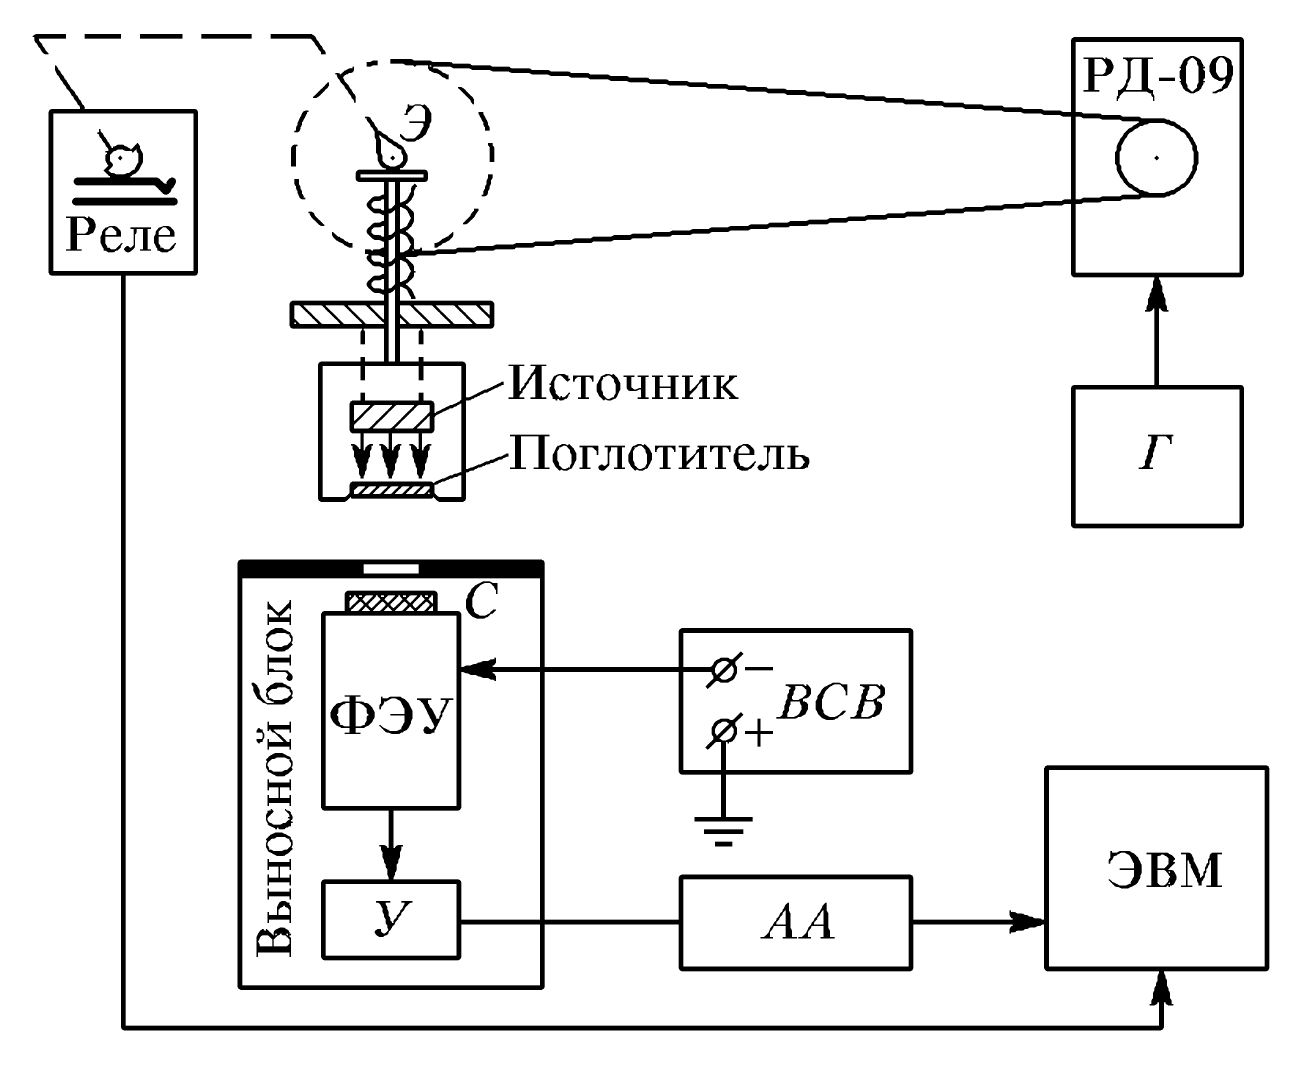
\includegraphics[width=0.7\linewidth]{lab}
		\caption{Блок-схема установки для наблюдения эффекта Мессбауэра: Э --- эксцентрик, С --- сцинтилляционный кристалл NaI(Tl), У --- усилитель, АА --- одноканальный амплитудный анализатор, ЭВМ --- персональный компьютер, $ \Gamma $ --- генератор для питания двигателя, Д-09 --- двигатель с редуктором, ВСВ --- высоковольтный стабилизированный выпрямитель}
		\label{lab}
	\end{figure}
	
	Изомер $^{119m}$Sn живет 250
	дней и распадается с излучением $ \gamma $-кван-
	тов с энергией 65 кэВ, переходя на короткоживущий первый возбужденный уровень.
	
	\begin{wrapfigure}[14]{l}{0.35\linewidth}
		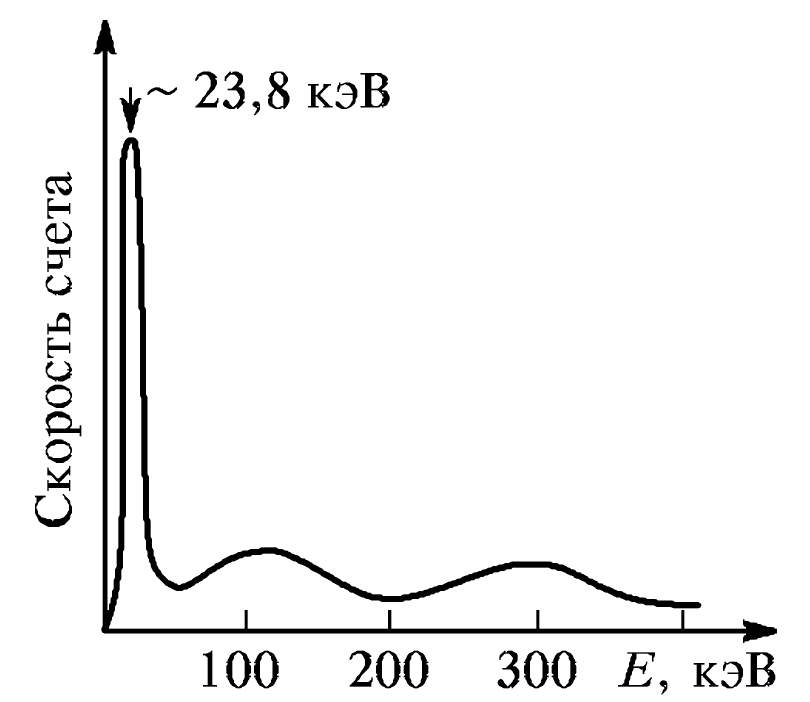
\includegraphics[width=\linewidth]{spek_lab}
		\caption{Спектр излучения источника BaSnO$_3 $, снятый с
			помощью сцинтилляционного спектрометра}
		\label{spek_lab}
	\end{wrapfigure}
	
	
	При каскадном переходе с первого
	уровня на основной излучаются используемые в работе $ \gamma $-лучи с энергией 23,8 кэВ.
	Источник получен в ядерном реакторе при
	облучении нейтронами образца олова, содержащего 96\% изотопа
	$ ^{118} $Sn. Переход с энергией 65 кэВ сильно конвертирован. Испускание электронов внутренней конверсии вызывает появление характеристического рентгеновского излучения с $ E_X = 25,4 $ кэВ. Это излучение образует "<фон">, мешающий измерениям. Этот фон можно значительно подавить с помощью характеристического фильтра
	из палладия. Край K-полосы поглощения палладия приходится на
	энергию $ E_K = 24,3 $ кэВ. Поэтому палладиевый фильтр сильно по-
	глощает рентгеновское излучение олова $ (E_X > E_K) $ и мало ослабляет поток исследуемых $ \gamma $-квантов ($ E_0 < E_K $). Палладиевая фольга
	толщиной 60 мкм приклеена непосредственно на источнике. Источник в металлическом контейнере укреплен неподвижно над поглотителем. Как правило, источники $ \gamma $-излучения содержат радиоактивные примеси, которые дают заметный вклад в суммарное излучение.

	На рис. \ref{spek_lab} показан спектр излучения источника BaSnO$_3 $, снятый с помощью калиброванного по энергии сцинтилляционного спектрометра с толстым (40 мм) кристаллом NaI(Tl). Максимумы в спектре
	соответствуют фотоэлектрическому поглощению $ \gamma $-квантов различных энергий в кристалле NaI(Tl). Они называются фотопиками (или
	пиками полного поглощения). В спектре источника кроме основной
	(мессбауэровской) линии $ \backsimeq 24 $ кэВ присутствуют кванты с энергиями $ \backsimeq $ 100 кэВ и $ \backsimeq  $ 300 кэВ. Для наблюдения эффекта необходимо выделить основную линию из общего излучения. Этого достигают, устанавливая "<окно"> амплитудного анализатора спектрометра на фотопик линии 23,8 кэВ.
	
	Данный спектрометр откалиброван заранее с помощью эталонных
	источников $ \gamma $-излучения. Если на ФЭУ подано напряжение, указанное на установке, то пик фотоэлектрического поглощения $ \gamma $-квантов с энергией 23,8 кэВ
	должен быть расположен в интервале значений порогов амплитудно-
	го анализатора от 1 до 10 В. Прошедшие через анализатор импульсы
	поступают для регистрации в ЭВМ.
	
	Канал счета времени и канал счета импульсов на ЭВМ выведены
	на реле, управление которым ведется от тефлоновых кулачков. Под их
	действием концевые выключатели замыкают или размыкают токовое
	питание электромагнита реле. Таким образом, схема автоматически
	включается на участке, где поглотитель движется с постоянной скоростью, и выключается, когда этот участок пройден. Скорость считается "<положительной">, если поглотитель движется навстречу источнику.
	При движении в обратном направлении скорость "<отрицательна">. При
	работе установки абсолютное значение скорости поглотителя указывается на дисплее ЭВМ, поскольку ЭВМ фиксирует время, за которое
	поглотитель проходит известный линейный участок.
	
	Смена скорости или ее подбор производится путем изменения частоты генератора, питающего двигатель; при этом следует также переключать согласующую емкость на двигателе. Диапазон изменения
	частоты --- от 0 до 200 Гц, а емкости --- от 0,1 до 0,4 мкФ. Чтобы вращать вал двигателя с большой скоростью, следует включать малую
	емкость и большую частоту. Для медленного вращения нужна малая
	частота и большая емкость. Измерять частоту и емкость при этом не нужно, так как скорость определяется путем независимого измерения,
	как это было указано выше.

	
	\section{Выполнение работы}
	
	Включив установку, проведем измерение спектра источника для определения фотопика $ \gamma $-квантов с энергией 23,8 кэВ. Для этого установим анализатор в режим фиксированного окна пропускания. Верхний порог задает ширину окна (0,5 В), а нижний будет задавать уровень, от которого окно отсчитывается. Изменяя значение нижнего порога от 0,5 до 9,5 В, занесем полученные результаты счета в секунду в таблицу \ref{table_5}. 
	
	Здесь и в дальнейшем ошибки измерения счета $ I $ будем считать по формуле ниже, с учетом того, что мы измеряем счет в течение 20 секунд:
	
	\begin{equation}\label{}
	\sigma_I = \sqrt{\dfrac{I}{20}}
	\end{equation}
	
	 \begin{table}[h]
	 	\caption{Излучение}
	 	\begin{center}
	 		\begin{tabular}{|c|c|c|c|}
	 			\hline
	 			$ N  $ & $ U $, В &  $ I, \; с^{-1} $ & $ \sigma_I, \; с^{-1} $  \\
	 			\hline
	 			2 & 0.5 & 15.6 & 0.88 \\
	 			3 & 1 & 10.2 & 0.71 \\
	 			4 & 1.5 & 14.6 & 0.85 \\
	 			5 & 2 & 49.6 & 1.57 \\
	 			6 & 2.5 & 84.6 & 2.06 \\
	 			7 & 3 & 84 & 2.05 \\
	 			8 & 3.5 & 123.4 & 2.48 \\
	 			9 & 4 & 152 & 2.76 \\
	 			10 & 4.5 & 187.6 & 3.06 \\
	 			11 & 5 & 183 & 3.02 \\
	 			12 & 5.5 & 169.8 & 2.91 \\
	 			13 & 6 & 100.4 & 2.24 \\
	 			14 & 6.5 & 65.6 & 1.81 \\
	 			15 & 7 & 29.6 & 1.22 \\
	 			16 & 7.5 & 10.8 & 0.73 \\
	 			17 & 8 & 5.4 & 0.52 \\
	 			18 & 8.5 & 4 & 0.45 \\
	 			19 & 9 & 3 & 0.39 \\
	 			20 & 9.5 & 3.4 & 0.41 \\
	 			\hline
	 		\end{tabular}
	 	\end{center}
	 	\label{table_5}
	 \end{table}
 
 Нанесем точки на график рис. \ref{graf_5} и профитируем его модифицировнной лоренцевой кривой \eqref{B-V}, которую мы зададим формулой
 	
 	\begin{equation}\label{yotx}
 y (x) = b - \dfrac{a}{1 + \left( \dfrac{x-X}{c/2}\right) ^2}
 \end{equation}
 
 	\begin{figure}[h]
 	\label{graf_5}
 	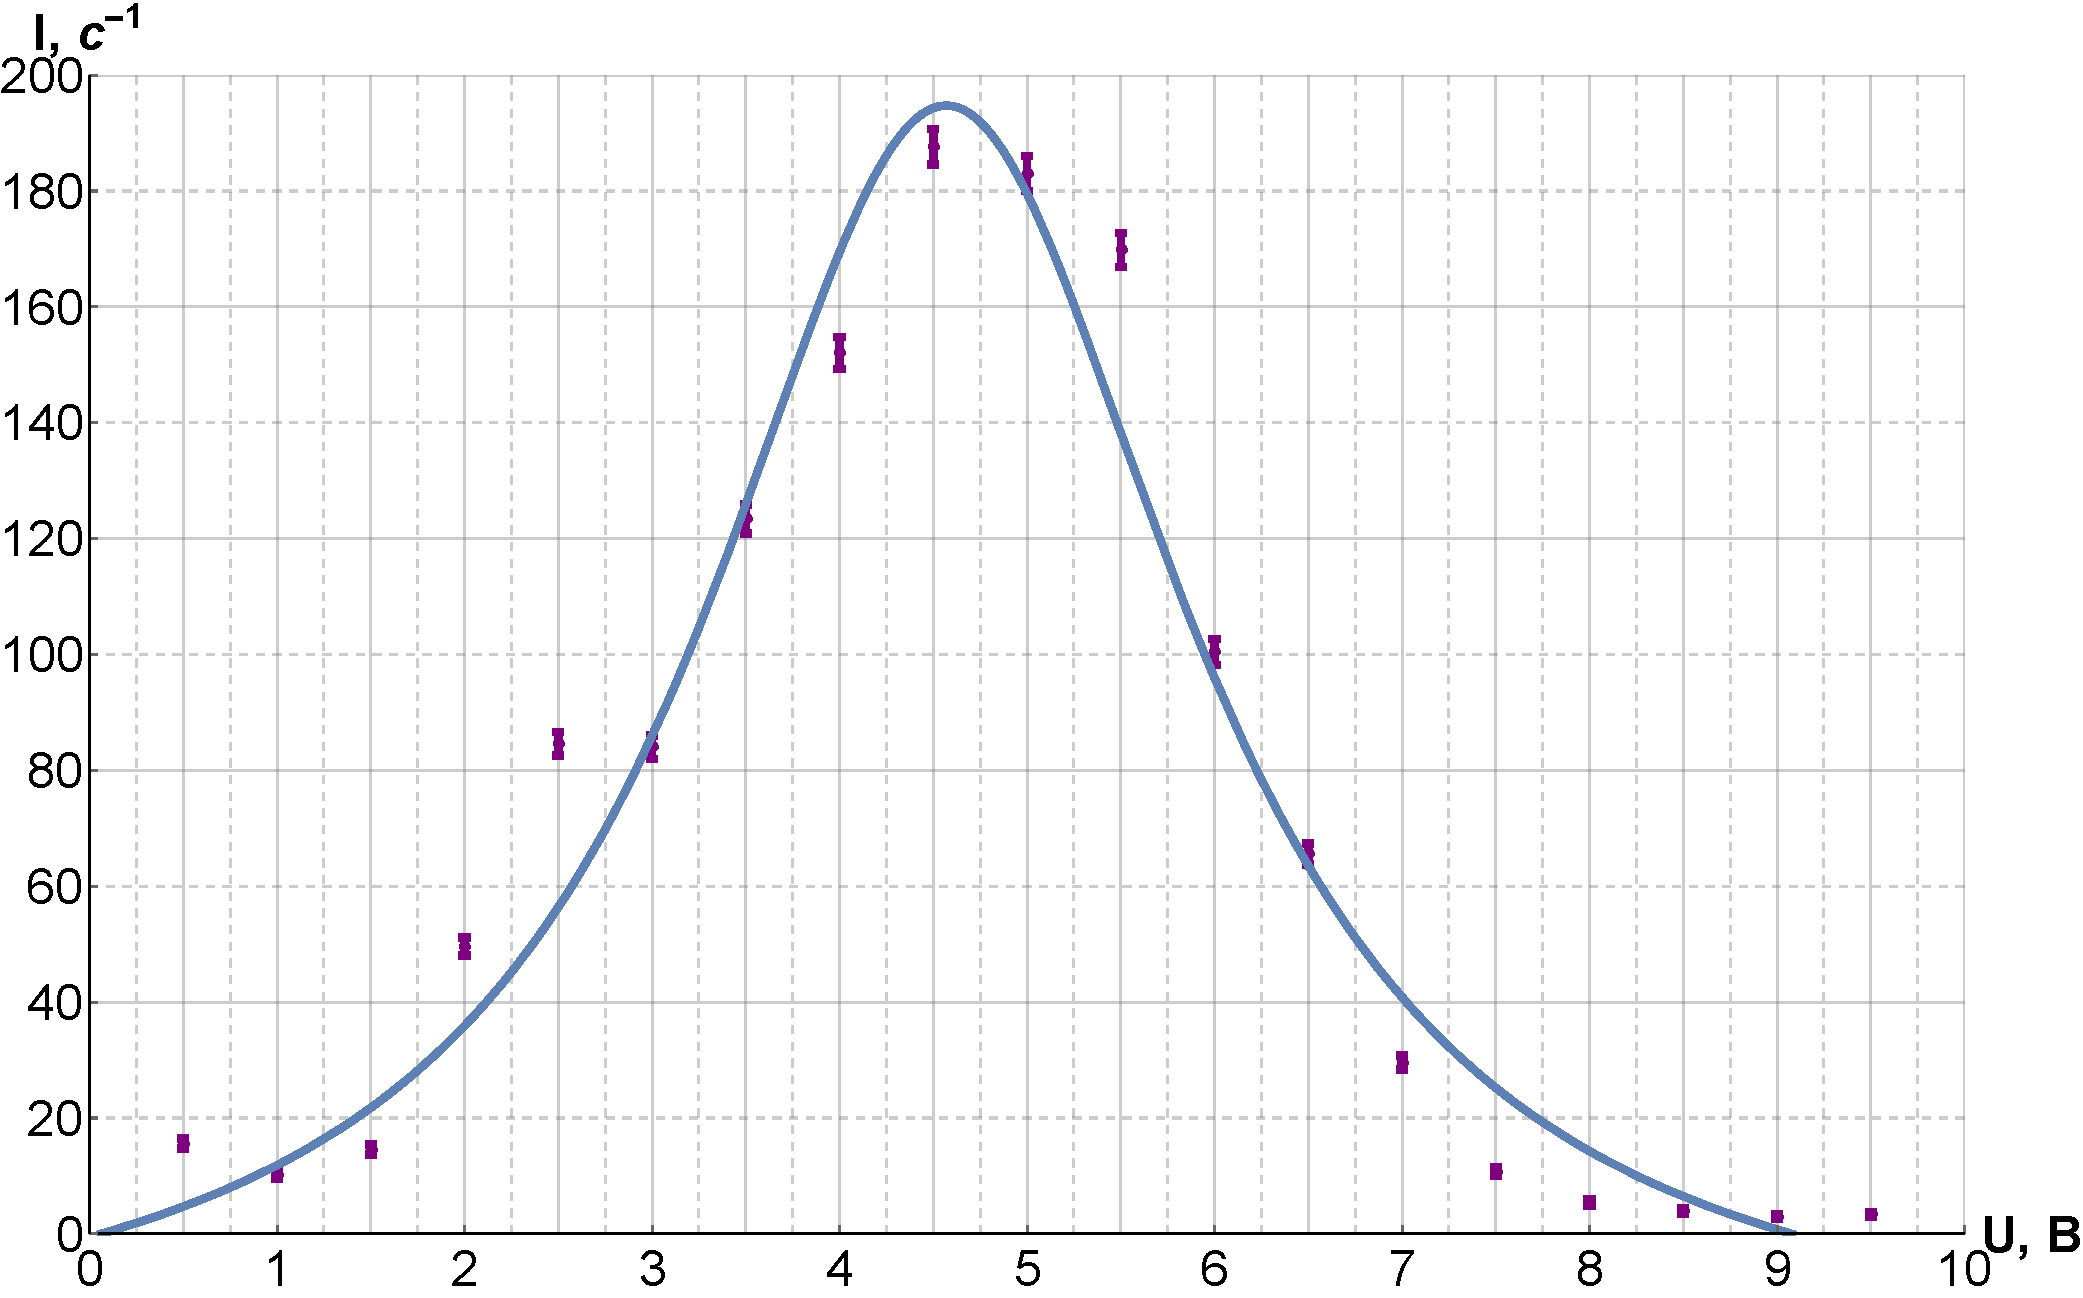
\includegraphics[scale=0.47]{gr5.pdf}
 	\caption{Излучение}
 \end{figure}
 
 	Теперь установим режим независимых значений порогов и установим их на 1,5 и 9 В. Перед измерением резонансного поглощения на образцах измерим скорость счета фон радиоактивного излучения. Она равна $ N_ф = 13,8 \; с^{-1} $.
 	
 	Теперь проведем измерения резонансного поглощения на 4-ех образцах: №1, №2, №3 --- это олово разной толщины, а №4 --- SnO$ _2 $. Результаты измерений занесем в таблицы \ref{table_1} -- \ref{table_4}. 
 	
 	Изобразим на графиках 6 -- 10 экспериментальные точки и профитируем их модицифировнной лоренцевой кривой \eqref{yotx}. Результаты всех 4-ех фитов сведем в таблицу \ref{table_fit}.
 	
 	 \begin{table}[h]
 		\caption{Результаты фитирования кривой резонансного поглощения}
 		\begin{center}
 			\begin{tabular}{|c|c|c|c|c|c|}
 				\hline
 				$ № $&  $ a  $ & $ b, \; с^{-1} $,  &  $ c, мм/c $ & $ X, мм/с $ & $ \chi_\nu^2 $ \\
 				\hline
 				1 & $ 103 \pm 6 $ & $ 990\pm 4 $ & 0,43 $\pm $ 0,04& $ 2,41 \pm 0,03 $ & 1,68 \\
 				2 & 114 $  \pm 5$ & \text{620 $  \pm $ 3} & \text{0,49 $  \pm $ 0,04} & \text{2,48 $ \pm $ 0,02} & 1,59\\
 				3 & \text{41 $  \pm  $ 3} & \text{163 $  \pm $ 1} & \text{0,58 $  $$ \pm $ 0,06} & \text{2,46 $ $$ \pm $ 0,03} & 1,43 \\
 				4 & \text{566$  $$ \pm $ 31} & \text{1580$  $$ \pm $ 5} & \text{0,78$  $$ \pm $ 0,05} & \text{-0,156$ 
 					$$ \pm $ 0,015} & 2,63\\
 				\hline
 			\end{tabular}
 		\end{center}
 		\label{table_fit}
 	\end{table}
 
 	Какой смысл полученных нами параметров фита? Нам пригодятся 3 из них: $ b $ --- величина фона, из которого мы "<вычитаем"> мэсбауэровский пик, $ 2с $ --- ширина резонансной линии $ \Gamma_{экс} $, а $ X $ --- величина химического сдвига. Под $ \chi_\nu^2 $ имеется ввиду критерий $ \chi^2 $, отнесенный к числу степеней свободны.
 
 	\begin{figure}[h]
 		\label{graf_1}
 		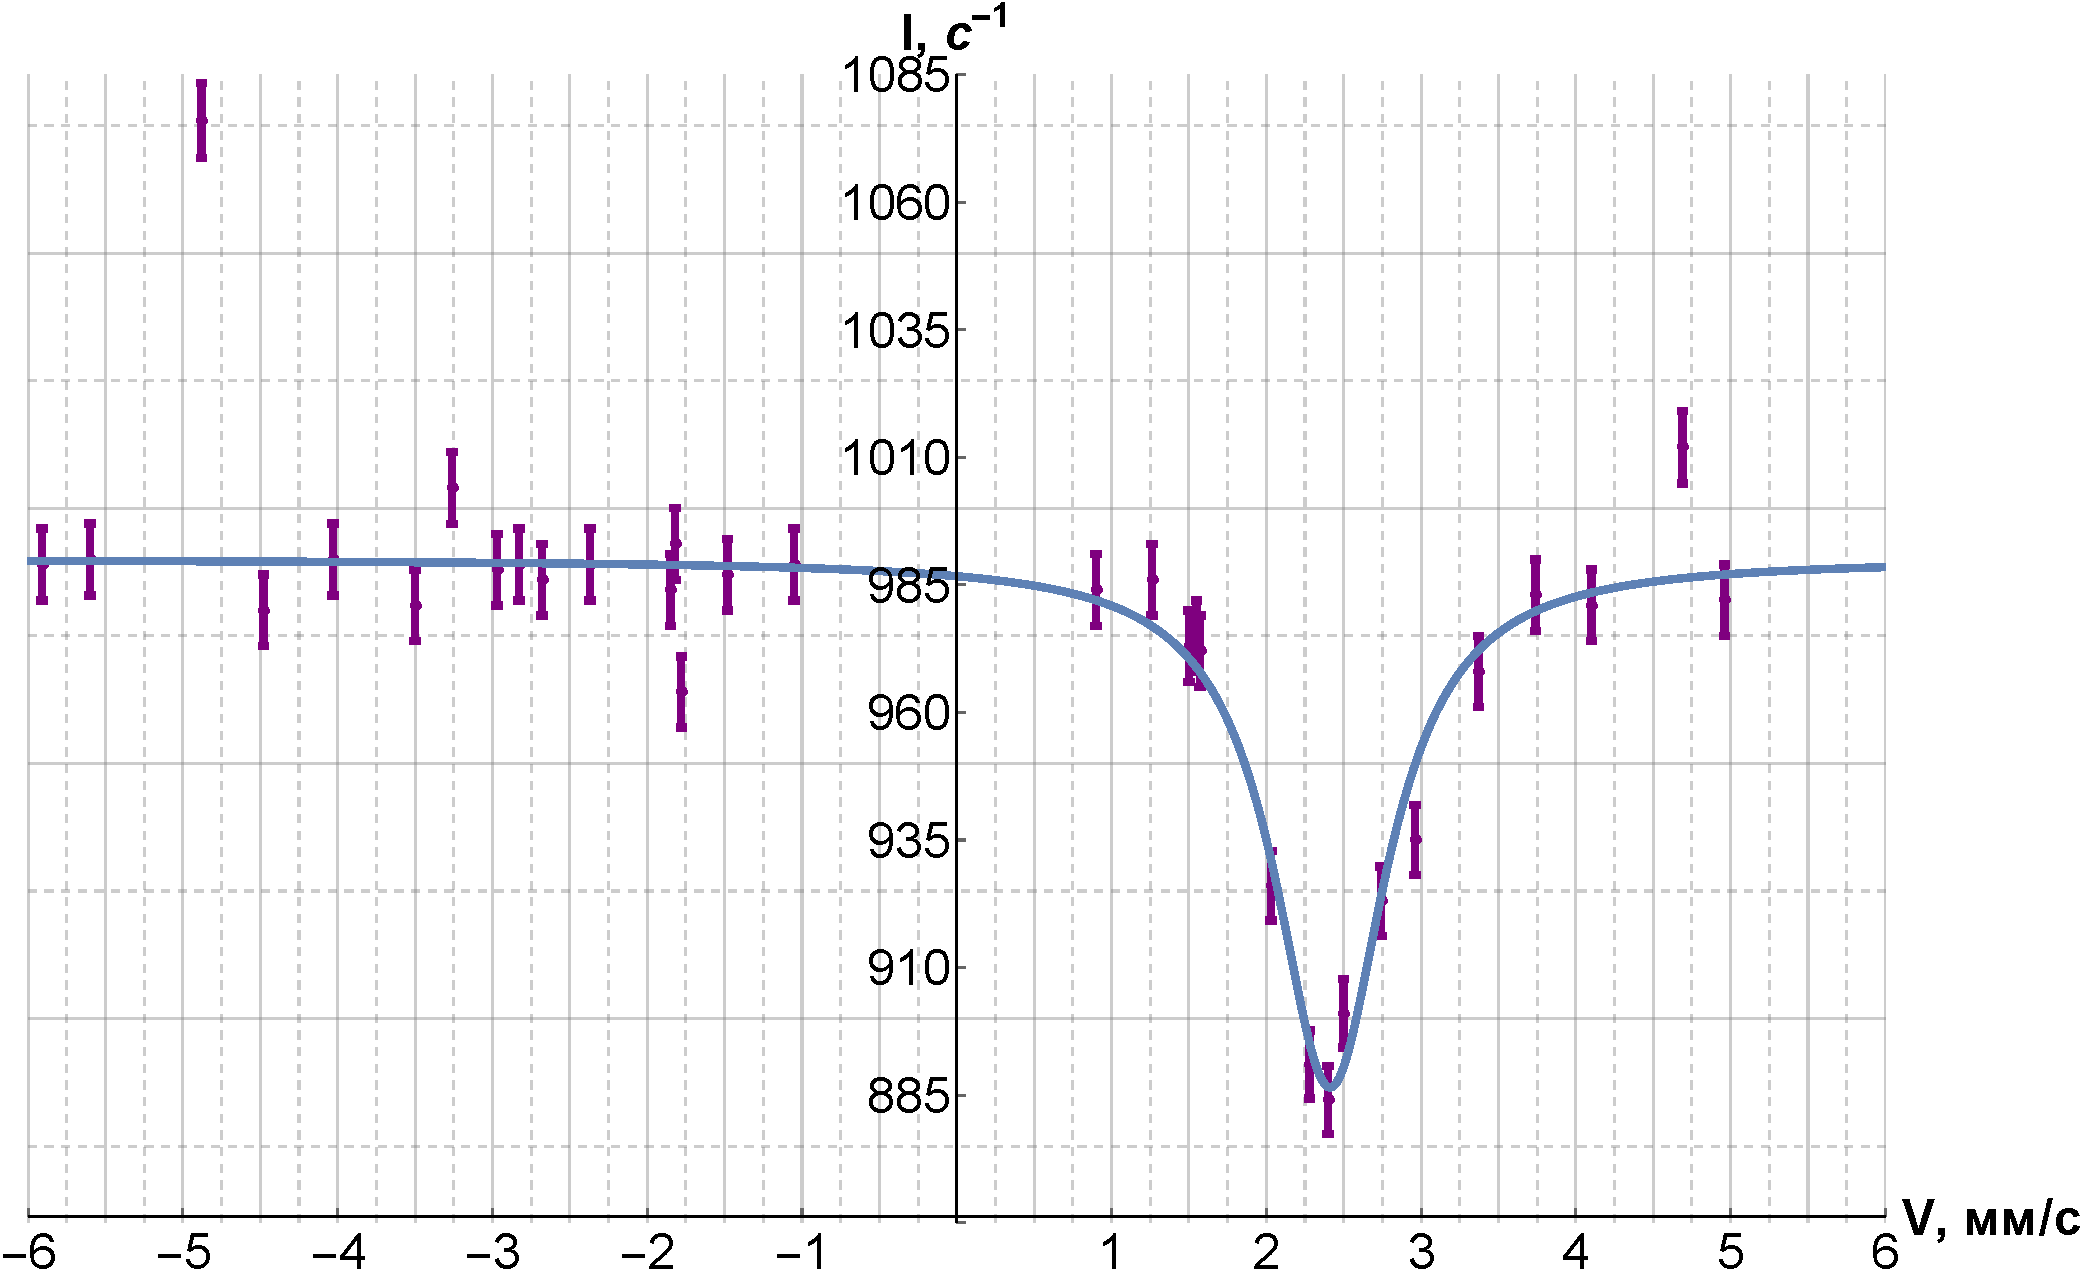
\includegraphics[scale=0.47]{gr1.pdf}
 		\caption{Резонансное поглощение на 1-ом поглотителе}
 	\end{figure}
 
 	\begin{figure}[h]
 		\label{graf_2}
 		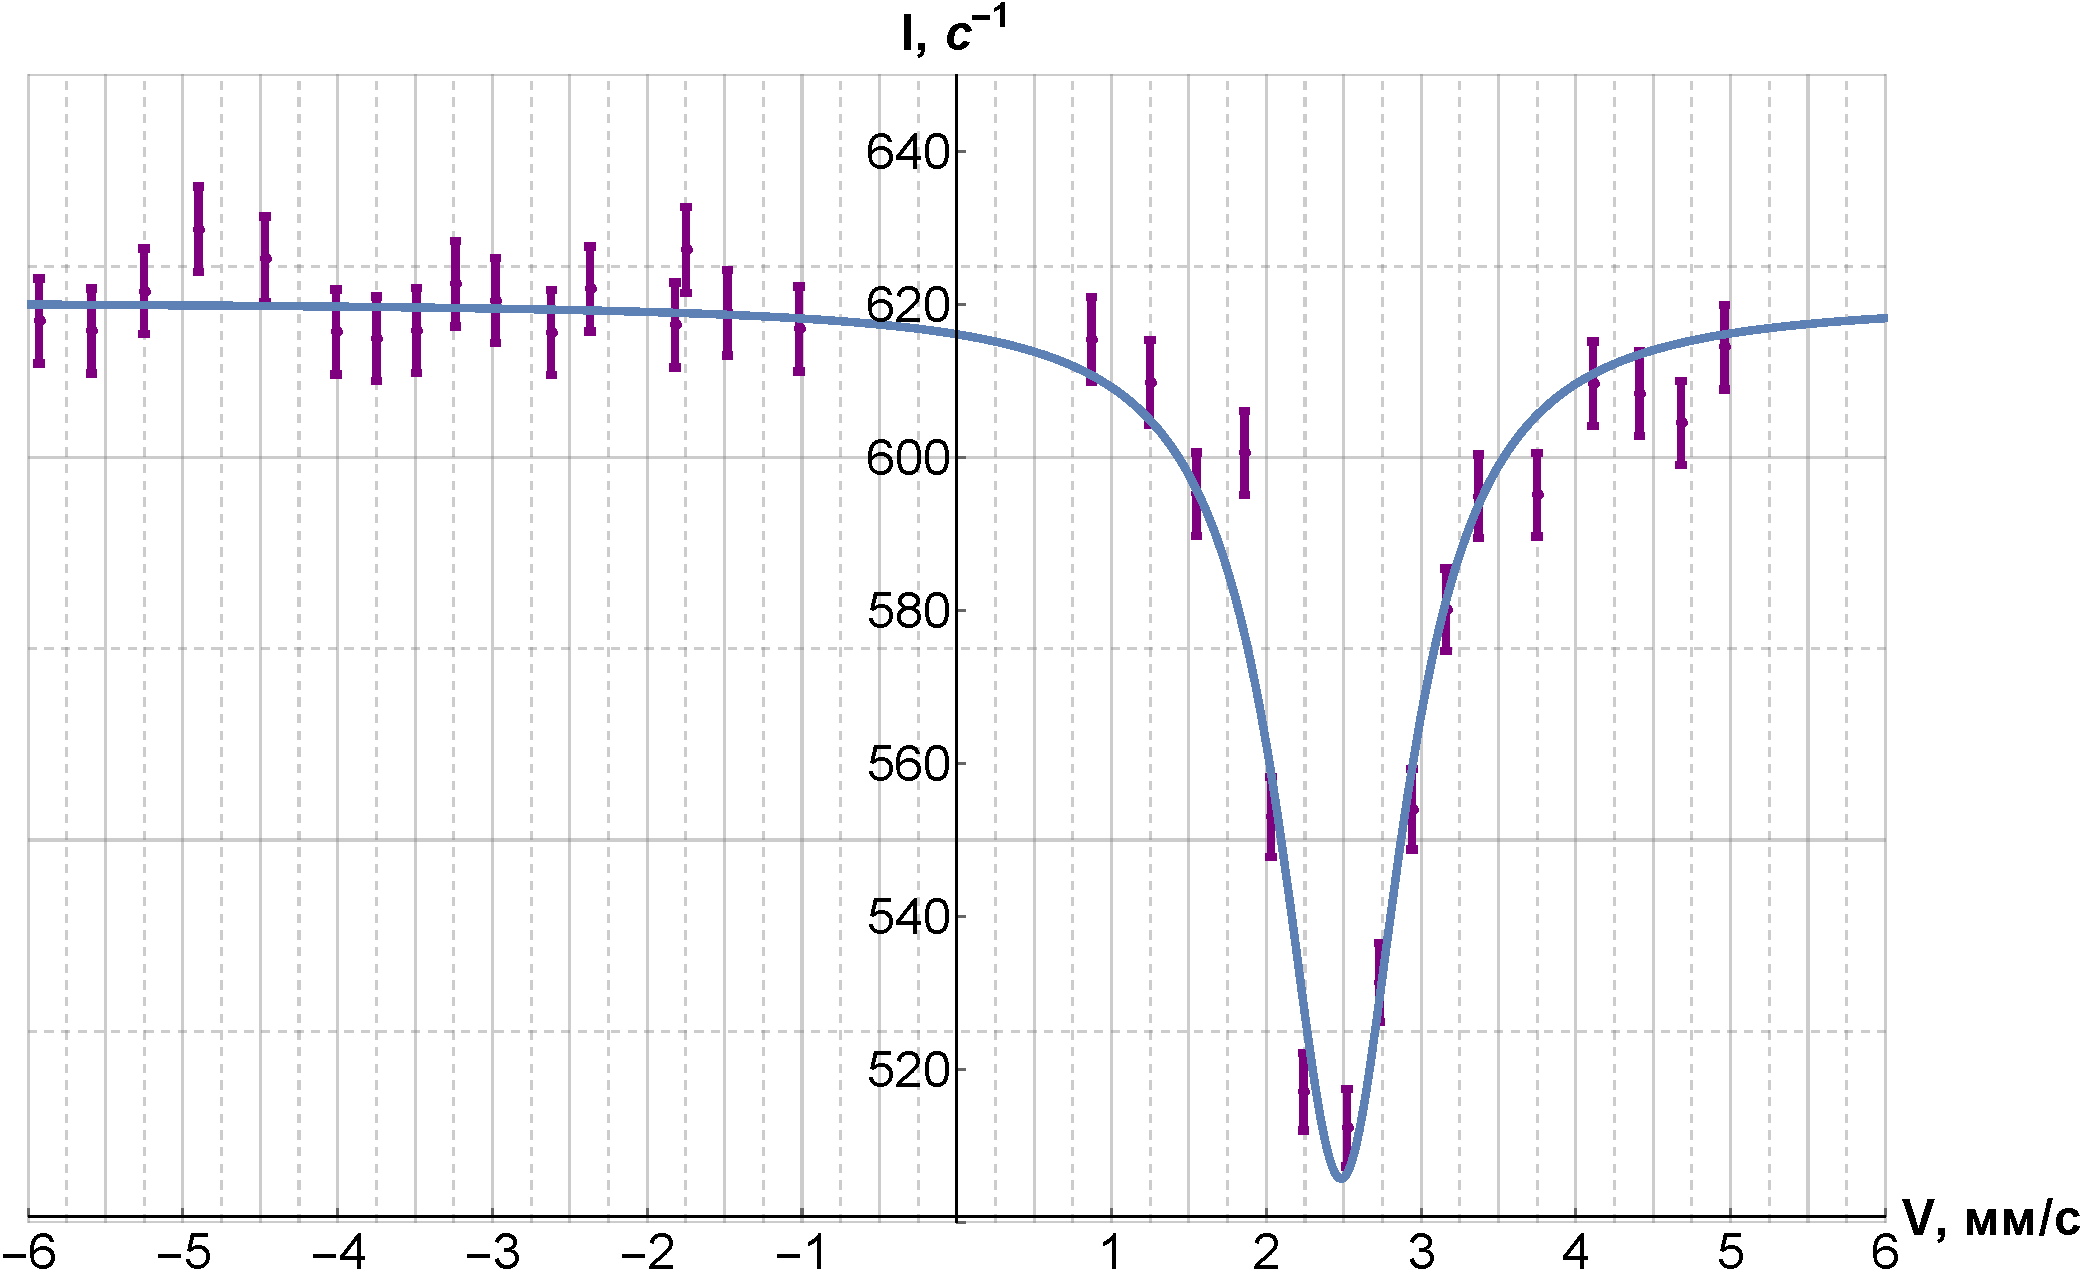
\includegraphics[scale=0.47]{gr2.pdf}
 		\caption{Резонансное поглощение на 2-ом поглотителе}
 	\end{figure}
 
 	\begin{figure}[h]
 		\label{graf_3}
 		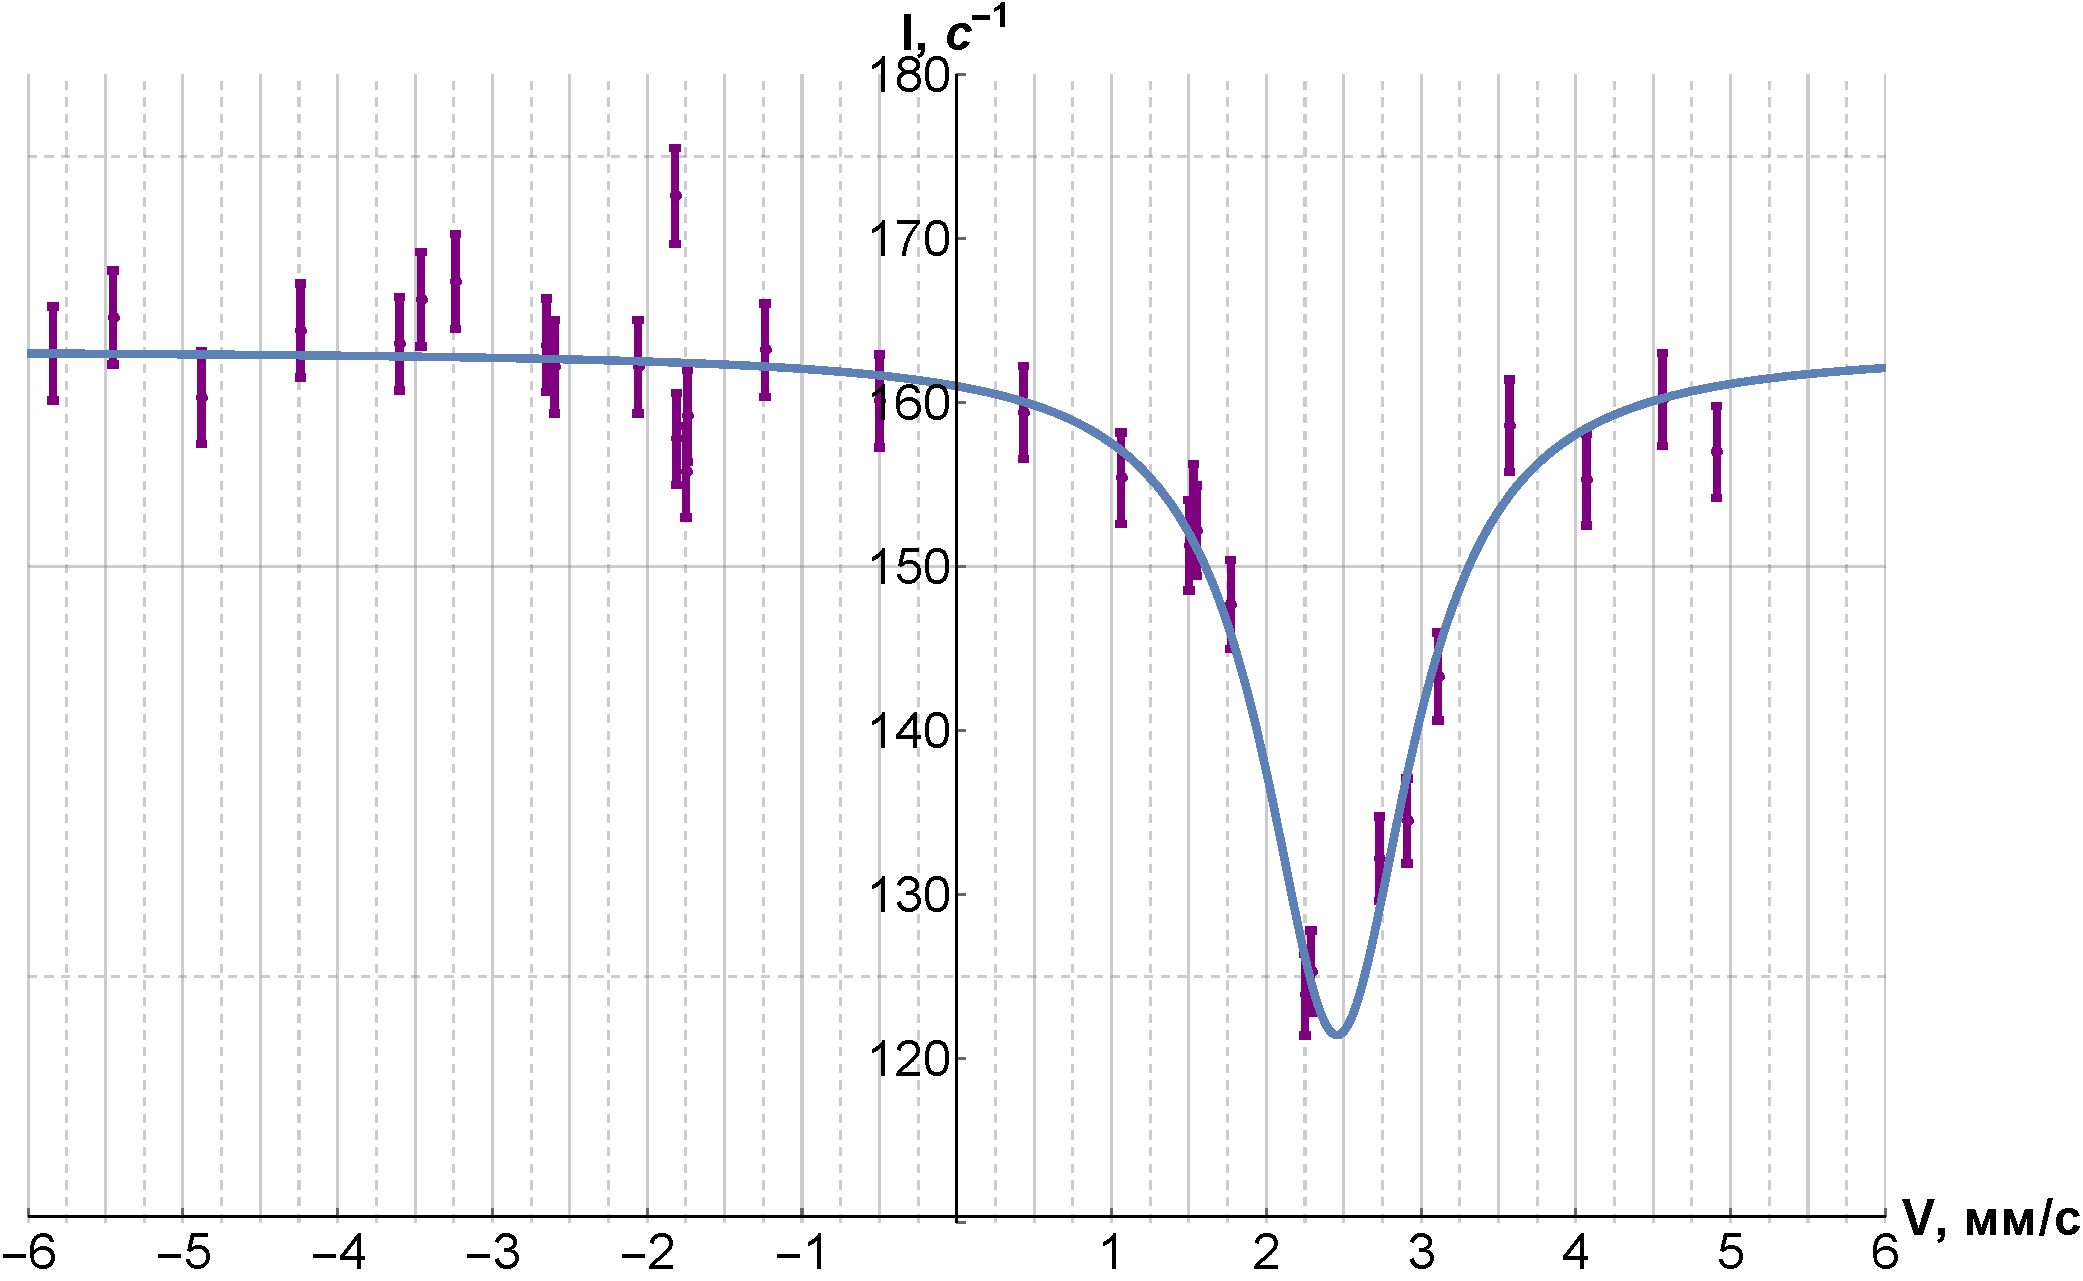
\includegraphics[scale=0.47]{gr3.pdf}
 		\caption{Резонансное поглощение на 3-ом поглотителе}
 	\end{figure}
 
 	\begin{figure}[h]
 		\label{graf_4}
 		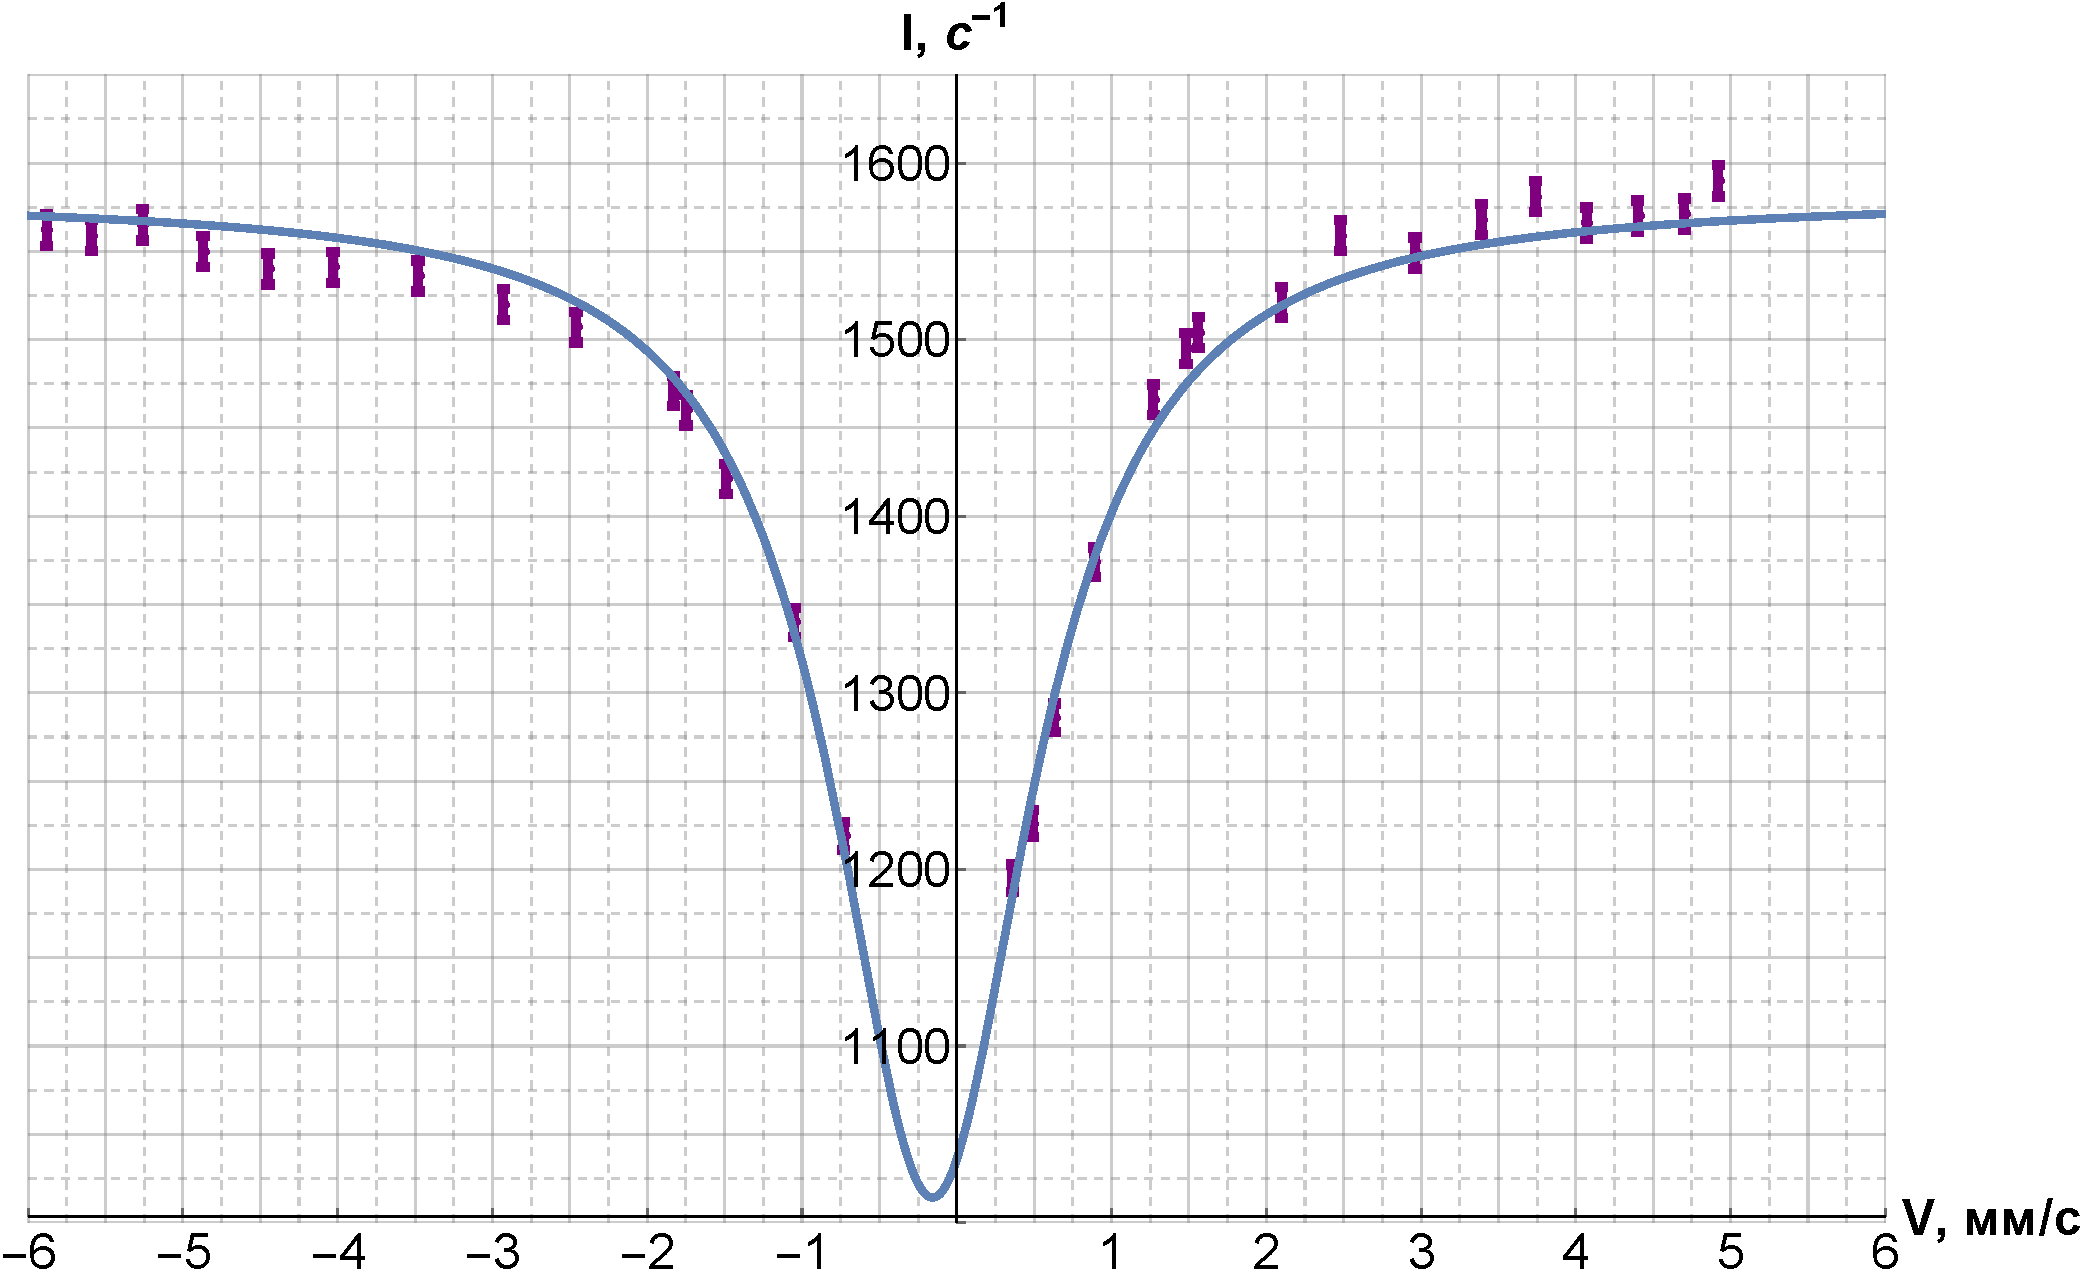
\includegraphics[scale=0.47]{gr4.pdf}
 		\caption{Резонансное поглощение на 4-ом поглотителе}
 	\end{figure}
 
 	На основе полученных результатов фитов мы можем вычислить амплитуды поглощения по формуле \ref{epsi;on}. Их погрешность оценим как
 	
 	\begin{equation}\label{ep}
 	\sigma_\epsilon = \epsilon \x \sqrt{\left( \dfrac{\sigma_{N_ф}}{N_ф} \right)^2 + \left( \dfrac{\sigma_{N(\infty)}}{N(\infty)} \right)^2 + \left( \dfrac{\sigma_{N(v)}}{N(v)} \right)^2 }
 	\end{equation}
 	
 	С учетом того, что $ N(\infty) = b, \; N(v) = y(X) $, мы можем подсчитать искомую величину. По формуле \eqref{D} мы можем оценить ширину уширения линии $  \Gamma_{экс} $ в эВ, подставляя как $ v = 2с , E_\gamma = 23,8 $ кэВ ($ c $ --- параметр фита).  Также из \eqref{vr} мы можем подсчитать химический сдвиг $ \Delta E $ в эВ, подставляя в качестве $ v_r = X $.  Вычисление параметров для всех поглотителей сведено в таблицу в выводе. Их погрешность вычислена через погрешности параметров фита аналогично \eqref{ep}.
 	
 	\section{Вывод}
 	
 	Результаты проделенной работы сведены в табличку. Мы измерили резонансное поглощение для четырех разных поглотителей и познакомились на их примере с эффектом Мэссбауэра. 
 	
  \begin{table}[h!]
 	\caption{Результаты работы}
 	\begin{center}
 	\begin{tabular}{|c|c|c|c|c|c|}
 		\hline 
 		№ & $\epsilon_i, \%$ & $ \Gamma_{экс}, мм/с $ & $  \Gamma_{экс}, 10^{-8} \x$ эВ & $ v_р, мм/с $ & $ \Delta E, 10^{-7}\x $, эВ \\ 
 		\hline 
 		1 & $ 10,6 \pm 0,9 $ & $ 0,86 \pm 0,08 $  & $ 7,3 \pm 0,6 $ & $ 2,41 \pm 0,03 $ & $ 1,91 \pm 0,02 $ \\ 
 		\hline 
 		2 &  $ 18,9 \pm 1,5 $& $ 0,98 \pm 0,09 $  & $  7,8 \pm 0,7 $ & $ 2,48 \pm 0,02 $ & $  1,97 \pm 0,01 $ \\ 
 		\hline 
 		3 & $ 28,1 \pm 0,9 $ & $ 1,116 \pm 0,12 $ & $  9,2 \pm 0,8 $ & $ 2,46 \pm 0,03 $ &  $ 1,95 \pm 0,02 $\\ 
 		\hline 
 		4 & $ 36,1 \pm 3,2 $  & $ 1,56 \pm 0,11 $ & $ 12,3 \pm 1,3  $ & $ -0,156 \pm 0,015 $ &  $ -0,123 \pm 0,006 $\\ 
 		\hline 
 	\end{tabular} 
 	\end{center}
\label{res}
\end{table}

Полученные результаты соотносятся с теоретическими расчетами. Уширение резонансной кривой по сравнению с $ 2\Gamma= 6\x10^{-8} $ эВ происходит при увеличении ширины поглотителя.
 
% \newpage
 \section*{Таблицы}
 
 
 \begin{table}[h!]
 	\caption{Измерения на 1-ом поглотителе}
 	\begin{center}
 		\begin{tabular}{|c|c|c|c|}
 			\hline
 			$ N  $ & $ v $, мм/с &  $ I, \; с^{-1} $ & $ \sigma_I, \; с^{-1} $  \\
 			\hline
 			1 & 4.96 & 982 & 7.01 \\
 			2 & 4.69 & 1012 & 7.11 \\
 			3 & 4.1 & 981 & 7 \\
 			4 & 3.74 & 983 & 7.01 \\
 			5 & 3.37 & 968 & 6.96 \\
 			6 & 2.96 & 935 & 6.84 \\
 			7 & 2.5 & 901 & 6.71 \\
 			8 & 2.03 & 926 & 6.8 \\
 			9 & 1.57 & 972 & 6.97 \\
 			10 & 1.5 & 973 & 6.97 \\
 			11 & 1.26 & 986 & 7.02 \\
 			12 & 0.9 & 984 & 7.01 \\
 			13 & 1.55 & 975 & 6.98 \\
 			14 & 2.74 & 923 & 6.79 \\
 			15 & 2.28 & 891 & 6.67 \\
 			16 & 2.4 & 884 & 6.65 \\
 			17 & -5.91 & 989 & 7.03 \\
 			18 & -5.6 & 990 & 7.04 \\
 			19 & -4.88 & 1076 & 7.33 \\
 			20 & -4.48 & 980 & 7 \\
 			21 & -4.03 & 990 & 7.04 \\
 			22 & -3.5 & 981 & 7 \\
 			23 & -2.97 & 988 & 7.03 \\
 			24 & -2.37 & 989 & 7.03 \\
 			25 & -1.85 & 984 & 7.01 \\
 			26 & -1.78 & 964 & 6.94 \\
 			27 & -1.48 & 987 & 7.02 \\
 			28 & -1.05 & 989 & 7.03 \\
 			29 & -1.82 & 993 & 7.05 \\
 			30 & -3.26 & 1004 & 7.09 \\
 			31 & -2.68 & 986 & 7.02 \\
 			32 & -2.83 & 989 & 7.03 \\
 			\hline
 		\end{tabular}
 	\end{center}
 	\label{table_1}
 \end{table}

	\begin{table}[h!]
		\caption{Измерения на 2-ом поглотителе}
		\begin{center}
			\begin{tabular}{|c|c|c|c|}
				\hline
				$ N  $ & $ v $, мм/с &  $ I, \; с^{-1} $ & $ \sigma_I, \; с^{-1} $  \\
				\hline
				1 & -5.93 & 617.8 & 5.56 \\
				2 & -5.59 & 616.5 & 5.55 \\
				3 & -5.25 & 621.7 & 5.58 \\
				4 & -4.9 & 629.8 & 5.61 \\
				5 & -4.47 & 625.9 & 5.59 \\
				6 & -4.01 & 616.4 & 5.55 \\
				7 & -3.49 & 616.6 & 5.55 \\
				8 & -2.98 & 620.5 & 5.57 \\
				9 & -2.37 & 622 & 5.58 \\
				10 & -1.82 & 617.3 & 5.56 \\
				11 & -1.75 & 627.1 & 5.6 \\
				12 & -1.48 & 618.9 & 5.56 \\
				13 & -1.02 & 616.8 & 5.55 \\
				16 & -3.24 & 622.7 & 5.58 \\
				17 & -2.62 & 616.3 & 5.55 \\
				18 & -3.75 & 615.5 & 5.55 \\
				19 & 4.96 & 614.4 & 5.54 \\
				20 & 4.68 & 604.5 & 5.5 \\
				21 & 4.41 & 608.3 & 5.51 \\
				22 & 4.11 & 609.6 & 5.52 \\
				23 & 3.75 & 595.1 & 5.45 \\
				24 & 3.37 & 594.9 & 5.45 \\
				25 & 2.94 & 554 & 5.26 \\
				26 & 2.52 & 512.4 & 5.06 \\
				27 & 2.03 & 553 & 5.26 \\
				28 & 1.55 & 595.2 & 5.46 \\
				29 & 1.86 & 600.6 & 5.48 \\
				30 & 1.25 & 609.8 & 5.52 \\
				31 & 0.87 & 615.4 & 5.55 \\
				32 & 2.73 & 531.4 & 5.15 \\
				33 & 2.24 & 517.1 & 5.08 \\
				34 & 3.16 & 580.1 & 5.39 \\
				\hline
			\end{tabular}
		\end{center}
		\label{table_2}
	\end{table}

	\begin{table}[h!]
		\caption{Измерения на 3-ом поглотителе}
		\begin{center}
			\begin{tabular}{|c|c|c|c|}
				\hline
				$ N  $ & $ v $, мм/с &  $ I, \; с^{-1} $ & $ \sigma_I, \; с^{-1} $  \\
				\hline
				1 & -5.84 & 163 & 2.85 \\
				2 & -5.45 & 165.2 & 2.87 \\
				3 & -4.88 & 160.3 & 2.83 \\
				4 & -4.24 & 164.4 & 2.87 \\
				5 & -3.46 & 166.3 & 2.88 \\
				6 & -2.65 & 163.5 & 2.86 \\
				7 & -1.75 & 155.8 & 2.79 \\
				8 & -1.24 & 163.2 & 2.86 \\
				9 & -0.5 & 160.1 & 2.83 \\
				10 & -1.82 & 172.6 & 2.94 \\
				11 & -2.06 & 162.2 & 2.85 \\
				12 & -2.6 & 162.2 & 2.85 \\
				13 & -3.24 & 167.4 & 2.89 \\
				16 & -3.6 & 163.6 & 2.86 \\
				17 & -1.81 & 157.8 & 2.81 \\
				18 & -1.74 & 159.2 & 2.82 \\
				19 & 4.91 & 157 & 2.8 \\
				20 & 4.56 & 160.2 & 2.83 \\
				21 & 4.07 & 155.3 & 2.79 \\
				22 & 3.57 & 158.6 & 2.82 \\
				23 & 2.91 & 134.5 & 2.59 \\
				24 & 2.25 & 123.9 & 2.49 \\
				25 & 1.5 & 151.3 & 2.75 \\
				26 & 1.06 & 155.4 & 2.79 \\
				27 & 0.43 & 159.4 & 2.82 \\
				29 & 1.77 & 147.7 & 2.72 \\
				30 & 2.29 & 125.3 & 2.5 \\
				31 & 2.73 & 132.2 & 2.57 \\
				32 & 3.11 & 143.3 & 2.68 \\
				33 & 1.55 & 152.2 & 2.76 \\
				34 & 1.53 & 153.5 & 2.77 \\
				\hline
			\end{tabular}
		\end{center}
		\label{table_3}
	\end{table}

	\begin{table}[h!]
		\caption{Измерения на 4-ом поглотителе}
		\begin{center}
			\begin{tabular}{|c|c|c|c|}
				\hline
				$ N  $ & $ v $, мм/с &  $ I, \; с^{-1} $ & $ \sigma_I, \; с^{-1} $  \\
				\hline
				1 & -5.88 & 1562 & 8.84 \\
				2 & -5.59 & 1559 & 8.83 \\
				3 & -5.26 & 1565 & 8.85 \\
				4 & -4.87 & 1550 & 8.8 \\
				5 & -4.45 & 1540 & 8.77 \\
				6 & -4.03 & 1541 & 8.78 \\
				7 & -3.48 & 1536 & 8.76 \\
				8 & -2.93 & 1520 & 8.72 \\
				9 & -2.46 & 1507 & 8.68 \\
				10 & -1.83 & 1471 & 8.58 \\
				11 & -1.75 & 1460 & 8.54 \\
				12 & -1.49 & 1421 & 8.43 \\
				13 & -1.05 & 1340 & 8.19 \\
				16 & -0.73 & 1219 & 7.81 \\
				17 & 4.92 & 1590 & 8.92 \\
				18 & 4.7 & 1571 & 8.86 \\
				19 & 4.4 & 1570 & 8.86 \\
				20 & 4.07 & 1566 & 8.85 \\
				21 & 3.74 & 1581 & 8.89 \\
				22 & 3.39 & 1568 & 8.85 \\
				23 & 2.96 & 1549 & 8.8 \\
				24 & 2.48 & 1559 & 8.83 \\
				25 & 2.1 & 1521 & 8.72 \\
				26 & 1.56 & 1504 & 8.67 \\
				27 & 1.48 & 1495 & 8.65 \\
				28 & 1.27 & 1466 & 8.56 \\
				29 & 0.89 & 1374 & 8.29 \\
				30 & 0.49 & 1226 & 7.83 \\
				31 & 0.36 & 1195 & 7.73 \\
				32 & 0.63 & 1286 & 8.02 \\
				\hline
			\end{tabular}
		\end{center}
		\label{table_4}
	\end{table}

	
\end{document}